
\providecommand{\myrootdir}{..}
\documentclass[\myrootdir/main.tex]{subfiles}

\begin{document}

\chapter{The Failing Build Logs Data Set}
\includegraphics[page=5, width=\textwidth, trim={0.5cm 0.5cm 0.5cm 0.5cm}, clip]{img/flow-of-research.pdf}

\label{data-set}
\section{Motivation}
originally: log collection to get impression of build logs from various projects, what possibly extractable information they contain and how strutured or unstructured they are.
Then labeling of one build log information, namely the reason the build failed, as well as keywords and stuructural category to use in our evaluation and support our impressions about suitability of the techniques with quantitative results

\section{Log Collector}
To collect a broad range of build logs we built the \texttt{Log Collector} using ruby.

  \subsection{Sampling Repositories}
  Our first task was to determine a set of repositories to query logs from. Our \texttt{GHTorrentParser} can query the GHTorrent dataset for the most popular languages on github and the most popular repositories for a given language. \emph{Popularity} in this case is defined as the number of watches. Our \texttt{TravisRequester} can then check for a given repository whether it uses Travis CI.

  \subsection{Sampling Builds}
  The \texttt{LogCollector} uses the \texttt{TravisRequester}, our tool querying the Travis API, to obtain the newest builds for a given repository. As most builds on Travis CI are successful \mention{citation needed} we use a stratified sampling approach: \texttt{TravisRequester} saves the found builds in logs in buckets according to their state. We encountered the following states during our data collection passes:
  \begin{itemize}
    \item \todo{fill /5 mins/}
  \end{itemize}
  \texttt{TravisRequester} saves up to a configured number of builds per state and searches through a configured number of maximum checked builds.

  \subsection{Sampling Logs}
  For each build the \texttt{TravisRequester} then selects a log to download. Logs in Travis CI are not directly attributed to \texttt{build}s, but to \texttt{job}s.
  A single build can consist of multiple jobs, e.g. building and executing tests in various different testing environments.
  \texttt{TravisRequester} therefore queries each build for a job, which has the same state.
  A failed build can have successful job executions, as just one failed job leads to the whole build being marked as failed.
  For the selected jobs, our tool then queries the Travis API V3 and obtains the respective build log.

\todo{image! like in travistorrent paper, /draft 10 mins/}

\section{Collection Process}
For our inital data collection to get an impression of build logs from various projects and languages we used the \texttt{LogCollector} to gather from the 30 most popular languages, up to 3 repositories using Travis CI each and 3 logs per state for each of those repositories.
For the \emph{Failing Build Log Data Set} we again collected from the same selection of repositories though saved only 10 logs of the state \emph{failed} for each repository.
our impression?
\todo{image!}

\section{Labeling (better name?)}
For our study, described in Chapter \ref{study}, we want to investigate the extraction capabilities of three techniques. Therefore, we need a data set of in/output examples for one \texttt{BuildLogInformation}. Furthermore, Keyword search is not configured by such in/output, but search keywords surrounding the desired output. Finally, this section describes our notion of structural categories, which we use to quantify our assumptions on the needed uniformness of in/output examples.

  \subsection{Build Failure Reason}

    \paragraph{Description}
    WHY? one common information developers and researches might want to extract, intentionally not focus on one structurally clearly defined extraction   cause that would be simple for PROSE extraction -> better comparability
    \paragraph{Labeling Process}

  \subsection{Keywords}

    \paragraph{Description}
    learning steps combining keywords -> similar to how devs would learn from reading those models

    \paragraph{Labeling Process}

  \subsection{Categories}

    \paragraph{Description}

    \paragraph{Labeling Process}

\section{Validation of our data set}
\todo{copy over from md doc}

\subsection{Inter-Rater Reliability}

\subsection{Sending Mails out to developers}

\end{document}
